\section{Results}
We reached several key insights from performing our
evaluations. First, we were able to discover hundreds of
censored websites that are not present on existing block
lists. Furthermore, we noticed that many websites on our block list
receive very little traffic. Lastly, we found that by using
politically-charged phrases as search terms, we were able to find a
disproportionally large amount of censored websites. The rest of this
section discusses the main findings in depth.

\subsection{Existing blocklists are incomplete}

\begin{figure*}[t]
  \centering
  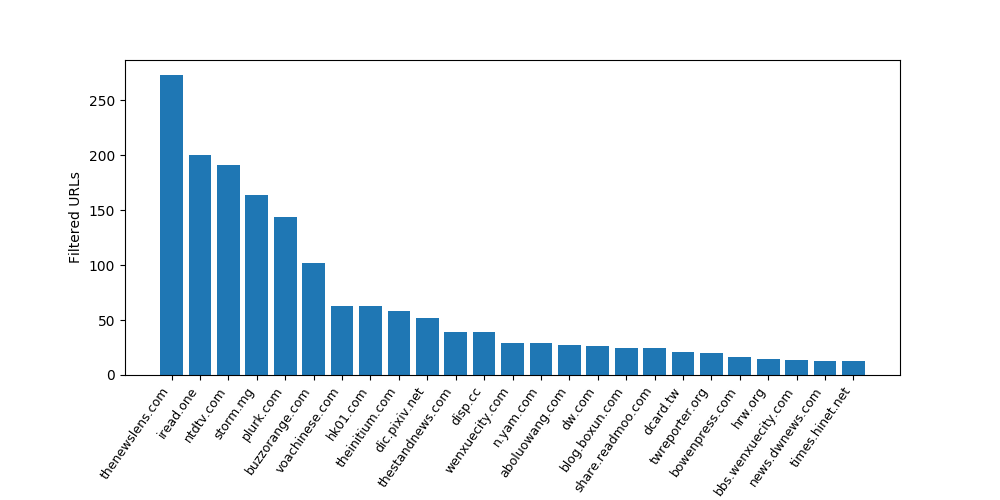
\includegraphics[scale=0.6]{figures/top-domains}
  \caption{\label{top-domains}Top censored domains by URL count.}
\end{figure*}

\begin{table}[b]
  \begin{center}
    \scalebox{0.80}{
    \begin{tabular}{ | l | r | r | r | }
      \hline
      Phrase length & Domains & Domains w/o Alexa Top 1000 \\ \hline
      Unigrams      & 1029    & 765 \\
      Bigrams       & 970     & 655 \\
      Trigrams      & 975     & 629 \\
      Total         & 1756    & \textbf{1125} \\
      \hline
    \end{tabular}}
  \end{center}
\caption{\label{breakdown} Total number of censored domains discovered.}
\end{table}

\textit{By using natural-language processing on Chinese webpages, we
were able to discover hundreds of censored websites that are not
present on the Citizen Lab block list--the standard for censorship
measurements--and FilteredWeb's block list~\cite{darer2017filteredweb,
citizenlab:block}}. Furthermore, the set of websites that appeared the
most in our search results is almost entirely different from that of
FilteredWeb. Figure~\ref{top-domains} breaks down this result when
using both bigrams and trigrams as search queries. These websites seem
to mainly cover Chinese human rights issues, news, and political
content.

For instance, \texttt{hrw.org} exposes a number of humans rights
issues in China, including the persecution of the Ugyhur minority
group~\cite{hrw:uighur}. Additionally, the \texttt{twreporter.org}
covers Taiwanese news, which may seem like an innocuous website to
Westerners. However, the relationship between Taiwan and China is
strained to the point that the Chinese government has attempted to
silence news outlets that report on Taiwan as its own
country~\cite{wapo:taiwan}. As such, the censorship of these popular
websites might reflect China's domestic and foreign policy.

Finally, only three of the top 25 domains that we discovered are in
the top 50 domain list produced by FilteredWeb. Four of the top five
domains that we discovered--\texttt{www.storm.mg},
\texttt{www.plurk.com}, \texttt{buzzorange.com}, and
\texttt{www.hk01.com}--are non-Western media websites that cover
Chinese news. These websites were also not present in the list of top
50 domains discovered by FilteredWeb. \textit{Thus, by building on the
approach of FilteredWeb, we were able to produce a qualitatively
different block list}. We recommend putting these two block lists
together to create a single block list that is both wide in scope and
large in size.

\begin{figure*}[t]
  \centering
  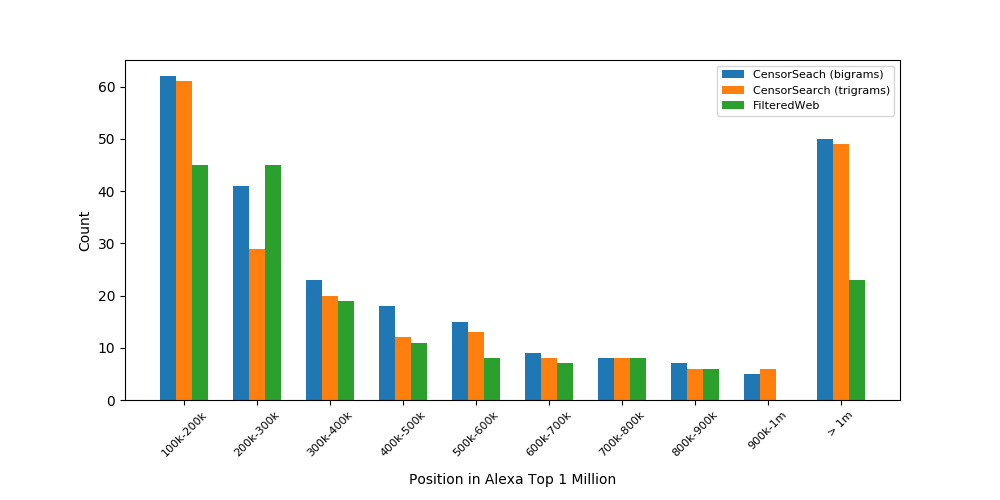
\includegraphics[scale=0.6]{figures/alexa}
  \caption{\label{alexa}Ranking of censored websites on Alexa Top 1 Million.}
\end{figure*}

\begin{figure}[b]
  \centering
  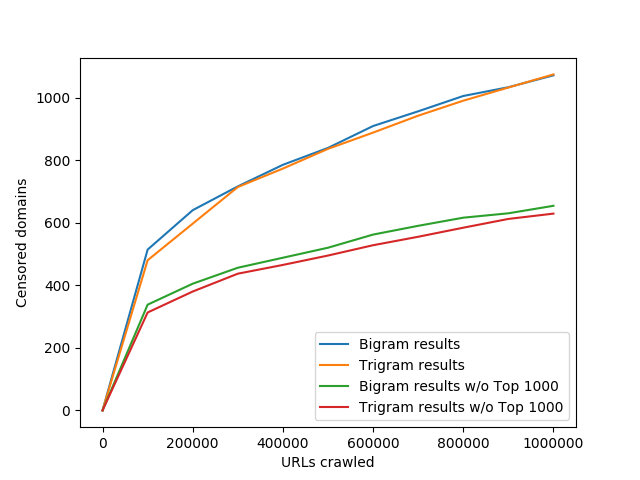
\includegraphics[scale=0.5]{figures/urls-crawled}
  \caption{\label{censored-vs-urls} Censored domains discovered over unique URLs crawled. }
\end{figure}

\subsection{China blocks many unpopular websites}

Figure~\ref{alexa} shows the ranking of the websites we discovered on
the Alexa Top 1,000,000. Notably, many of the websites we discovered
are spread throughout the tail of the list, and some of the websites
are not even on the list at all. \textit{Given that the top 100,000 websites
likely receive the vast majority of traffic on the Internet, we can
infer that censors in China are not just interested in blocking
``big-name'', popular websites.} They are actively seeking out websites
of \textit{any size} that contain ``sensitive'' content. We also
discovered a number of websites that fall outside the Alexa Top
1,000,000 altogether. Without the use of an automated systen that can
discover censored websites, it's unlikely that the public would even
be aware that these websites are blocked.

Furthermore, we were able to consistently discover \textit{more} unpopular
censored domains with our approach than FilteredWeb. For domains that
rank between 200,000 and 300,000 on the Alexa Top 1,000,000,
FilteredWeb was able to discover more domains, but in every other bin of
100,000 ranks we discovered more. Notably, between the ranks of 900,000
and 1,000,000, FilteredWeb did not discover \textit{any} censored domains, and
we discovered far more domains that fall outside of the Alexa Top
1,000,000 altogether. This suggests that the use of Chinese phrases
as search queries allowed us to uncover a significant number of
websites that would otherwise be unknown to censorship researchers.

Lastly, Table \ref{breakdown} shows the breakdown of how many censored
websites we discovered. By using bigrams, we were able to discover 964
censored domains that are not on any publicly available block list,
655 of which are outside the Alexa Top 1000. Similarly, by using
trigrams, we were able to discover 969 domains that are not on any
publicly available block list, 629 of which are outside the Alexa Top
1000. In total, we found 1,405 domains, 757 of which are outside of
the Alexa Top 1000~\cite{alexa:top1000}. Each of these evaluations
were performed with 1,000,000 unique URLs, consistent with the
methodology of FilteredWeb~\cite{darer2017filteredweb}. Figure \ref{censored-vs-urls} shows how
many censored domains we discovered as a function of unique URLs
crawled for each evaluation.

\begin{table*}[t]
  \begin{center}
    \scalebox{0.9}{
      \begin{tabular}{ l | l | c }
        Chinese & English & Censored domains \\ \hline
        \begin{CJK*}{UTF8}{gbsn}王歧山\end{CJK*} & Wang Qishan & 74\% \\
        \begin{CJK*}{UTF8}{gbsn}李洪志\end{CJK*} & Li Hongzhi & 64\% \\
        \begin{CJK*}{UTF8}{gbsn}郭伯雄\end{CJK*} & Guo Boxiong & 62\% \\
        \begin{CJK*}{UTF8}{gbsn}胡锦涛\end{CJK*} & Hu Jintao & 56\% \\
        \begin{CJK*}{UTF8}{gbsn}胡平\end{CJK*}  & Hu Ping & 54\% \\
        \begin{CJK*}{UTF8}{gbsn}Morty\end{CJK*} & Morty & 52\% \\
        \begin{CJK*}{UTF8}{gbsn}命案\end{CJK*}  & Homicide & 52\% \\
        \begin{CJK*}{UTF8}{gbsn}特首\end{CJK*}  & Chief executive & 52\% \\
        \begin{CJK*}{UTF8}{gbsn}Vimeo\end{CJK*} & Vimeo & 50\% \\
        \begin{CJK*}{UTF8}{gbsn}中情局\end{CJK*} & CIA & 50\% \\
      \end{tabular}}
  \end{center}
  \caption{\label{effective-unigrams}Sample of unigrams with
    significant blockrates}
\end{table*}

\begin{table*}[t]
  \begin{center}
    \scalebox{0.9}{
      \begin{tabular}{ l | l | c }
        Chinese & English & Censored domains \\ \hline
        \begin{CJK*}{UTF8}{gbsn}中共\end{CJK*} \begin{CJK*}{UTF8}{gbsn}威胁\end{CJK*} & Chinese Communists threaten & 50\% \\
        \begin{CJK*}{UTF8}{gbsn}声明的\end{CJK*} \begin{CJK*}{UTF8}{gbsn}反共产主义\end{CJK*} & Declared anti-communist & 44\% \\
        \begin{CJK*}{UTF8}{gbsn}中国共\end{CJK*} \begin{CJK*}{UTF8}{gbsn}产党的公共安全\end{CJK*} & Public security of the CPC & 42\% \\
        \begin{CJK*}{UTF8}{gbsn}北京\end{CJK*} \begin{CJK*}{UTF8}{gbsn}清洁\end{CJK*} & Beijing clean-up & 40\% \\
        \begin{CJK*}{UTF8}{gbsn}江泽民\end{CJK*} \begin{CJK*}{UTF8}{gbsn}胡锦涛\end{CJK*} & Jiang Zemin Hu Jintao & 40\% \\
        \begin{CJK*}{UTF8}{gbsn}迫害\end{CJK*} \begin{CJK*}{UTF8}{gbsn}活动\end{CJK*} & Persecution
                                                     activities & 40\% \\
        \begin{CJK*}{UTF8}{gbsn}官员\end{CJK*} \begin{CJK*}{UTF8}{gbsn}呼吁\end{CJK*} & Officials called on & 36\% \\
        \begin{CJK*}{UTF8}{gbsn}重的\end{CJK*} \begin{CJK*}{UTF8}{gbsn}公民\end{CJK*} & Heavy Citizen & 36\% \\
        \begin{CJK*}{UTF8}{gbsn}非法\end{CJK*} \begin{CJK*}{UTF8}{gbsn}拘留\end{CJK*} & Illegal detention
                          & 36\% \\
        \begin{CJK*}{UTF8}{gbsn}不同\end{CJK*} \begin{CJK*}{UTF8}{gbsn}的民主\end{CJK*} & Different Democratic & 34\% \\
      \end{tabular}}
  \end{center}
  \caption{\label{effective-bigrams}Sample of bigrams with significant
    block rates}
\end{table*}

\begin{table*}[t]
  \begin{center}
    \scalebox{0.9}{
      \begin{tabular}{ l | l | c }
        Chinese & English & Censored domains \\ \hline
        \begin{CJK*}{UTF8}{gbsn}北戴\end{CJK*} \begin{CJK*}{UTF8}{gbsn}河\end{CJK*} \begin{CJK*}{UTF8}{gbsn}会议\end{CJK*} & BEIDAIHE meeting & 54\% \\
        \begin{CJK*}{UTF8}{gbsn}中国\end{CJK*} \begin{CJK*}{UTF8}{gbsn}共产党\end{CJK*} \begin{CJK*}{UTF8}{gbsn}的宗教政策\end{CJK*} & The Chinese Communist Party's religious policy & 42\% \\
        \begin{CJK*}{UTF8}{gbsn}采取\end{CJK*} \begin{CJK*}{UTF8}{gbsn}暴力\end{CJK*} \begin{CJK*}{UTF8}{gbsn}镇压\end{CJK*} & To take a violent crackdown & 38\% \\
        \begin{CJK*}{UTF8}{gbsn}香港\end{CJK*} \begin{CJK*}{UTF8}{gbsn}政\end{CJK*} \begin{CJK*}{UTF8}{gbsn}治\end{CJK*} & Hong Kong Politics & 34\% \\
        \begin{CJK*}{UTF8}{gbsn}欧洲\end{CJK*} \begin{CJK*}{UTF8}{gbsn}议会\end{CJK*} \begin{CJK*}{UTF8}{gbsn}决议\end{CJK*} & European Parliament Resolution & 32\% \\
        \begin{CJK*}{UTF8}{gbsn}新\end{CJK*} \begin{CJK*}{UTF8}{gbsn}唐\end{CJK*} \begin{CJK*}{UTF8}{gbsn}王朝\end{CJK*} & New Tang Dynasty & 32\% \\
        \begin{CJK*}{UTF8}{gbsn}恐怖\end{CJK*} \begin{CJK*}{UTF8}{gbsn}事件\end{CJK*} \begin{CJK*}{UTF8}{gbsn}。\end{CJK*} & A terrorist event. & 32\% \\
        \begin{CJK*}{UTF8}{gbsn}天安\end{CJK*} \begin{CJK*}{UTF8}{gbsn}门广\end{CJK*} \begin{CJK*}{UTF8}{gbsn}场示威\end{CJK*} & Tiananmen Square Demonstrations & 32\% \\
        \begin{CJK*}{UTF8}{gbsn}敦促\end{CJK*} \begin{CJK*}{UTF8}{gbsn}美国\end{CJK*} \begin{CJK*}{UTF8}{gbsn}政府\end{CJK*} & Urging the US government & 32\% \\
        \begin{CJK*}{UTF8}{gbsn}1989\end{CJK*} \begin{CJK*}{UTF8}{gbsn}民主\end{CJK*} \begin{CJK*}{UTF8}{gbsn}运动\end{CJK*} & 1989 democracy movement & 30\% \\
      \end{tabular}}
  \end{center}
  \caption{\label{effective-trigrams}Sample of trigrams with
    significant blockrates}
\end{table*}

\subsection{Political phrases are highly effective}
\label{phrases-eval}

We also wanted to see if there is a correlation between the
presence of certain phrases and whether or not a given website is
censored.  For example, if we make a search
for \begin{CJK*}{UTF8}{gbsn}中国侵犯人权\end{CJK*} (Chinese human
rights violation) and find that a particular search result is
censored, then we cannot be certain whether the presence of that phrase
\textit{caused} the website to be blocked. Even if we assume 
that a censor is manually combing through search engines to find
sensitive websites, the website could have been blocked because it
contained totally different content.

Nevertheless, there seems to be some correlation for both bigrams and
trigrams. Table~\ref{effective-bigrams} shows a sample of bigrams
that returned the most number of unique filtered domains from
Bing. There are a couple of things to note. First, most of the bigrams
refer to the Chinese Communist Party in some
way. Phrases such as \begin{CJK*}{UTF8}{gbsn}中共的威胁\end{CJK*}
(Chinese Communists threaten), \begin{CJK*}{UTF8}{gbsn}江泽民胡锦
涛\end{CJK*} (Jiang Zemin Hu Jintao), and \begin{CJK*}{UTF8}{gbsn}中国
共产党的治安\end{CJK*} (Public security of the CPC) do not necessarily
convey sensitive information, but they nonetheless refer to the
government of China. On the other hand, some phrases clearly refer to
political dissent, such as \begin{CJK*}{UTF8}{gbsn}官员呼吁\end{CJK*}
(Officials called on), \begin{CJK*}{UTF8}{gbsn}迫害活动\end{CJK*}
(Persecution activities), \begin{CJK*}{UTF8}{gbsn}非法拘留\end{CJK*}
(Illegal detention), and \begin{CJK*}{UTF8}{gbsn}宣称反共\end{CJK*}
(Declared anti-communist).

Table~\ref{effective-trigrams} shows a sample of trigrams
that returned the most number of unique filtered domains from
Bing. Phrases that stand out include \begin{CJK*}{UTF8}{gbsn}中国共产
党的宗教政策\end{CJK*} (The Chinese Communist Party's religious
policy), \begin{CJK*}{UTF8}{gbsn}天安门广场示威\end{CJK*} (Tiananmen
Square demonstrations), \begin{CJK*}{UTF8}{gbsn}1989年民主运
动\end{CJK*} (1989 democracy movement), and \begin{CJK*}{UTF8}{gbsn}采
取暴力镇压\end{CJK*} (To take a violent crackdown). Interstingly, we
also see that discussion of China's religious
policy, the ``New Tang Dynasty''--a religious radio broadcast located in
the United States--, and European Union legislation may also be
considered sensitive content.~\cite{china-religion}. \textit{Together,
these results suggest that references to collective political
dissent are highly likely to be censored}. This
is consistent with the findings of King et al.~\cite{king2013censorship}.